\documentclass{article}
\usepackage[T1]{fontenc}

\usepackage{graphicx}
\usepackage{listings}
\begin{document}

\title{FOSS Lab Report}
\author{Gokul K\\[2\baselineskip]
Roll Number: 21\\[2\baselineskip]}
\date{02 February 2020}

\maketitle

\setcounter{section}{15}
\section{Shell Programming XII}
\subsection{Aim}
Write a shell script that displays a list of all the files in the current
directory to which the user has read, write and execute permissions.


\subsection{Source Code}
\begin{verbatim}
    #! /bin/bash

    # Gokul K
    # Roll No: 21
    # 25-01-2020

    # Write a shell script that displays a list of all the files in the current
    # directory to which the user has read, write and execute permissions.

    ls -l | grep "^-rwx" | awk '{printf "%s",$NF; printf "\n"}'

\end{verbatim}

\subsection{Program Description}
Regular Expression pattern "\^-rwx" searches for words starting with -rwx which\newline
corresponds to all the files current user has read, write and execute permissions.\newline
Hence when piped to ls -l only lines corresponding to those files will be printed. Hence\newline
with awk we can select only the filenames to output

\subsection{Output}
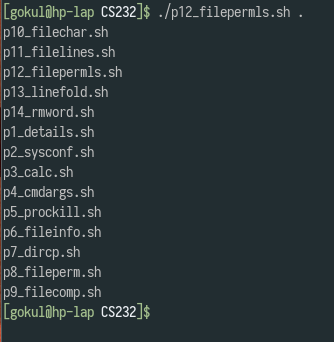
\includegraphics[width=0.9\textwidth]{img/p16.png}\newline

\subsection{Result}
The above program is run on Manjaro Linux shell. All files where user
has rwx permissions is obtained as output
\end{document}